\section{Prérequis et environnement de développement}
Dans cette partie, je présentai les outils et technologies utiliser durant le processus de développement du projet.\\

\subsection{Matériels}

\subsubsection{Arduino Uno}

\begin{figure}[H]
  \centering
  \href{https://www.arduino.cc/en/main/arduinoBoardUno}{
  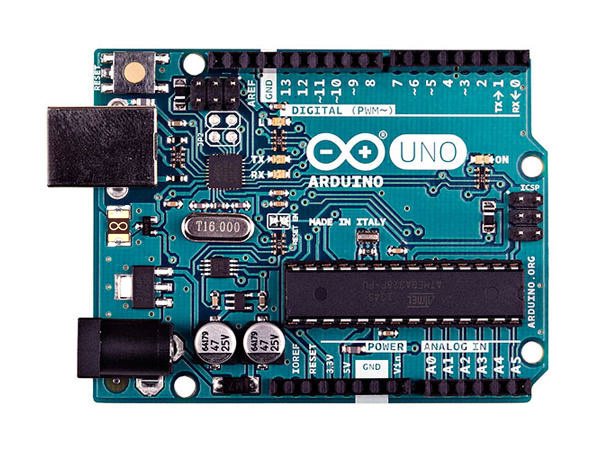
\includegraphics[width=7cm]{image/arduino_uno.jpg}
    }
  \caption{Microcontrôleur Arduino Uno}
\end{figure}

Arduino/Genuino Uno est un microcontrôleur  basé sur le soc ATmega328P. Il a 14 pins entrée/sortie pins (dont 6 qui peuvent être utilisés comme prise de courant 5v), 6 entrées analogiques, 16 MHz de fréquence, une connexion USB, une prise de courant, une tête ICSP et un bouton remise a zéro.\\

\subsubsection{Shield WiFi Arduino}

\begin{figure}[H]
  \centering
  \href{https://www.arduino.cc/en/Main/ArduinoWiFiShield}{
  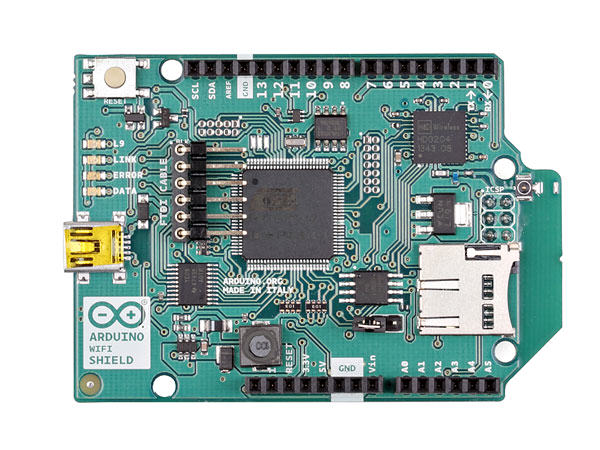
\includegraphics[width=7cm]{image/arduino_wifi.jpg}
  }
  \caption{Shield Wifi Arduino}
\end{figure}

L'Arduino WiFi Shield\footnote{"Bouclier" en anglais, c'est une carte conçue pour et ajouter des fonctionnes se poser sur l'Arduino} permet de relié l'Arduino à Internet sans fil.

\begin{itemize}
\item Nécessite un Arduino pour fonctionner.
\item Tension de service 5V (fournie par la carte Arduino). 
\item Arduino Due compatible.
\item Connexion via: réseaux 802.11b/g.
\item Types de cryptage: WEP et WPA2 personnels.
\item Connexion avec Arduino sur le port SPI.
\item Slot micro SD embarqué.
\item En-têtes ICSP.
\item Connexion FTDI pour le débogage en série du bouclier WiFi.
\item mini-USB pour la mise à jour du micrologiciel du bouclier WiFi.
\end{itemize}




\subsubsection{Shield bluetooth Arduino}

\begin{figure}[H]
  \centering
  \href{https://www.seeedstudio.com/Seeed-BLE-Shield-p-1859.html}{
  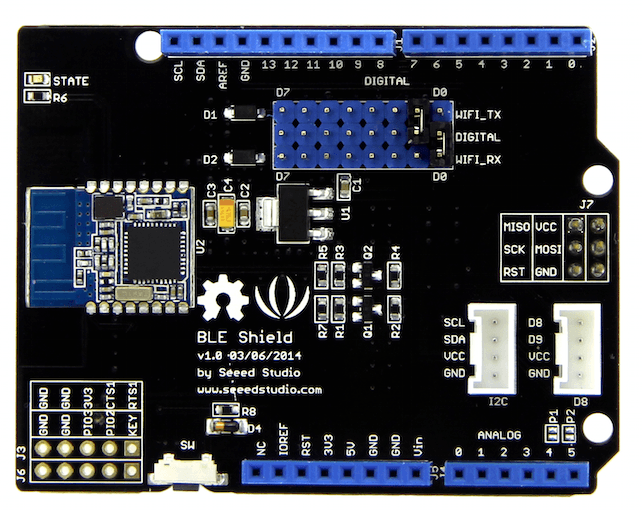
\includegraphics[width=7cm]{image/arduino_ble.png}
  }
  \caption{Shield Bluetooth Arduino}
\end{figure}

Le Bluetooth Shield intègre un module Serial Bluetooth. Il peut être facilement utilisé avec Arduino pour une communication série sans fil transparente. on peut  choisir deux broches d'Arduino D0 à D7 en tant que Ports Serial\footnote{ Transmission série} Serial pour communiquer avec Bluetooth Shield (D0 et D1 est Hardware Serial Port). La shield comporte également deux connecteurs \href{https://www.seeedstudio.com/Grove-Universal-4-pin-connector-p-789.html}{Grove}  (l'un est numérique, l'autre est analogique) pour installer des modules Grove.



\subsubsection{Capteurs de gaz MQ2, MQ6, MQ8}

\begin{figure}[H]
  \centering
  \href{http://playground.arduino.cc/Main/MQGasSensors}{
  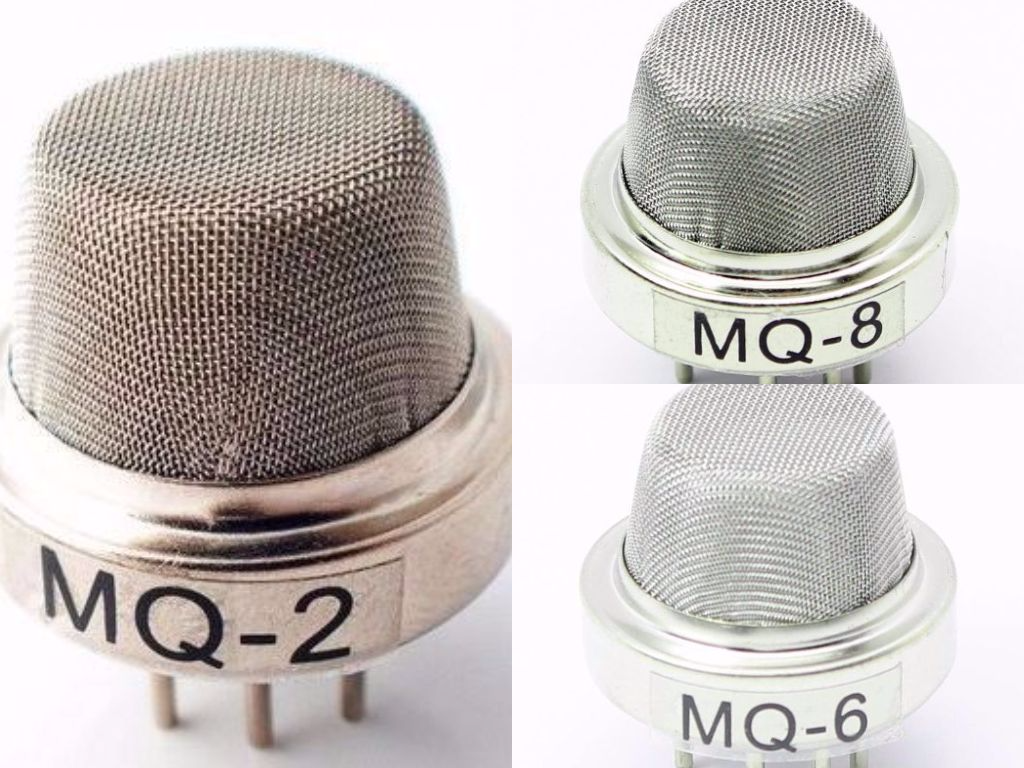
\includegraphics[width=7cm]{image/mq.png}
  }
  \caption{Capteurs de gaz MQ2,MQ6,MQ8}
\end{figure}

\begin{itemize}
\item Le capteur MQ2 peut être utilisé pour la détection de H2, LPG\footnote{Liquefied petroleum gas}, CH4, CO, Alcool, fumée ou Propane. 
\item Le capteur MQ6 peut être utilisé pour la détection de LPG ou CH4. 
\item Le capteur MQ8 peut être utilisé pour la détection de H2.

\end{itemize}


%sec%
\subsubsection{ESP8266}

\begin{figure}[H]
  \centering
  \href{https://fr.wikipedia.org/wiki/ESP8266}{
  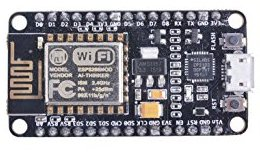
\includegraphics[width=7cm]{image/esp8266.png}
  }
  \caption{ESP8266-12E}
\end{figure}

L’ESP8266 est un circuit intégré à microcontrôleur avec connexion Wifi développé par le fabricant chinois \href{https://espressif.com/}{Espressif}.\\
Voici ses caractéristiques techniques:\\
\begin{itemize}

\item 32-bit RISC CPU: Tensilica Xtensa LX106, 80 MHz 64 KiB d’instructions RAM, 96 KiB de RAM de données.
\item QSPI flash externe - 512 KiB jusqu’à 4 MiB (support jusqu’à 16 MiB), IEEE 802.11 b/g/n Wifi.
\item TR switch intégré, balun\footnote{Un balun est un circuit électrique utilisé pour effectuer la liaison entre : une ligne de transmission symétrique (ligne bifilaire ou lignes imprimées parallèles) et une ligne de transmission asymétrique (câble coaxial ou ligne imprimée au-dessus d'un plan de masse)}, LNA, amplificateur de signal Wifi et compatibilité avec les réseaux WEP or WPA/WPA2, 16 GPIO pins ,SPI, I2C,I2S interfaces avec DMA (partage de pins avec GPIO).
\item UART dans les pins dédies , 10-bit ADC.
\end{itemize}

J’ai présenté en haut les matériels le plus importants pour la réalisation du projet, il y a toute la connectique derrière que je ne présenterai pas dans ce rapport.


\subsection{Logiciels}

\subsubsection{Arduino IDE}

\begin{figure}[H]
  \centering
  \href{https://www.arduino.cc/en/main/software}{
  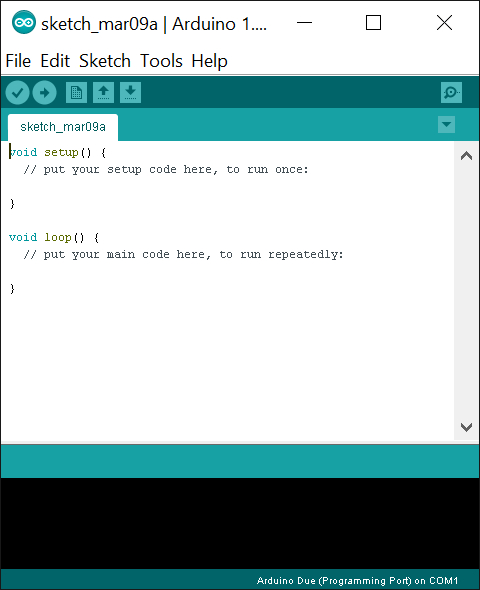
\includegraphics[width=8cm,height=8cm]{image/arduino_ide.png}
  }
  \caption{Arduino Web IDE}
\end{figure}
L'IDE est bon pour un début mais ensuite, je me suis rendu compte qu'il est pas assez puissant lors de la phase de débogage.
J'ai opté pour  la solution Arduino Cmake qui est parfaite pour les besoins de mon projet.

\subsubsection{Arduino CMake}

Arduino est une plate-forme de développement formidable, facile à utiliser. Il a tout ce dont un débutant devrait avoir besoin. L'IDE Arduino simplifie beaucoup de choses pour l'utilisateur standard, mais si vous êtes un programmeur professionnel, l'IDE peut paraître simpliste et restrictif.

Un inconvénient majeur de l'IDE d'Arduino est que je ne peux rien faire sans celui-ci, ce qui pour moi est une destruction totale. C'est pourquoi j'ai utilisé un système de construction alternatif pour Arduino.

\href{https://github.com/queezythegreat/arduino-cmake}{CMake} est un excellent système de construction multiplateforme qui fonctionne sur pratiquement n'importe quel système d'exploitation. Avec cela, on n'est pas contraint à un seul système de construction. CMake me permet de générer le système de construction qui correspond à mes besoins. Il peut générer tout type de système de construction, à partir de simples Makefiles, pour compléter des projets pour Eclipse, Visual Studio, XCode, etc.

Le système de construction Arduino CMake s'intègre étroitement au SDK Arduino qui doit être installé au préalable (Si l'IDE Arduino est installé sur la machine implique que le SDK est déjà installé sur votre système).

Pour pouvoir compiler sous Linux il faudra avoir les logiciel suivant sur la machine de développement  :

\begin{itemize}
\item gcc-avr - AVR GNU GCC compilateur 
\item binutils-avr - AVR outils binaire
\item avr-libc - AVR C librairie
\item avrdude - utiliser pour charger le firmware.
\end{itemize}


\subsubsection{Espruino IDE}

Espruino est un interpréteur JavaScript pour les microcontrôleurs. Il est conçu pour les appareils dotés d'un flash de 128kB et d'une RAM de 8kb.

\begin{figure}[H]
  \centering
  \href{https://www.espruino.com/}{
  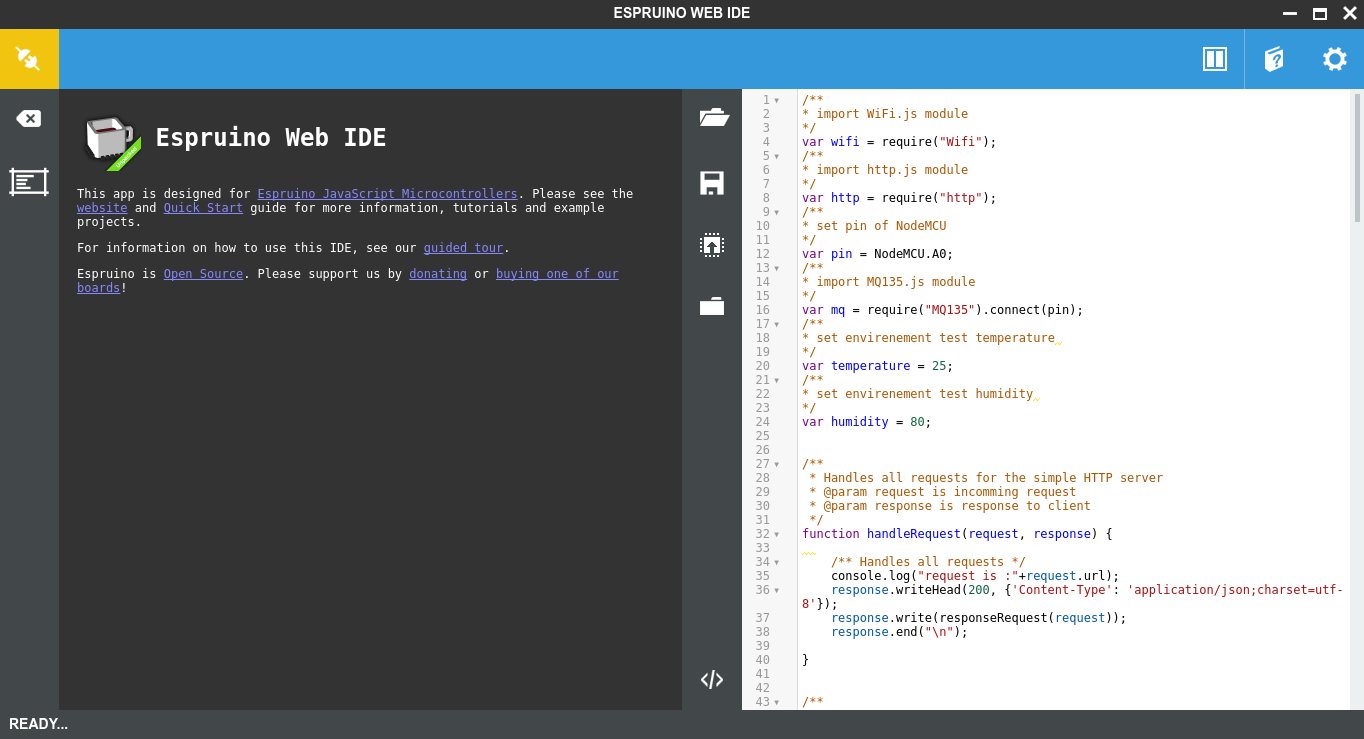
\includegraphics[width=15cm]{image/web00.png}
  }
  \caption{Espruino Web IDE}
\end{figure}

L'IDE peut être intégré au navigateur Chrome ou Chromium (version open source de chrome) sous la forme d'une extension qu'on peut installer du Chrome \href{https://chrome.google.com/webstore/detail/espruino-web-ide/bleoifhkdalbjfbobjackfdifdneehpo}{web store} ou à partir du dépôt \href{https://github.com/espruino/EspruinoWebIDE}{GitHub}  officiel.  

il est disponible également sous la forme d'un module \href{https://www.npmjs.com/package/espruino}{Node.js}  pour les puristes de la ligne de commande.

\begin{figure}[H]
  \centering
  \href{https://github.com/espruino/EspruinoTools}{
  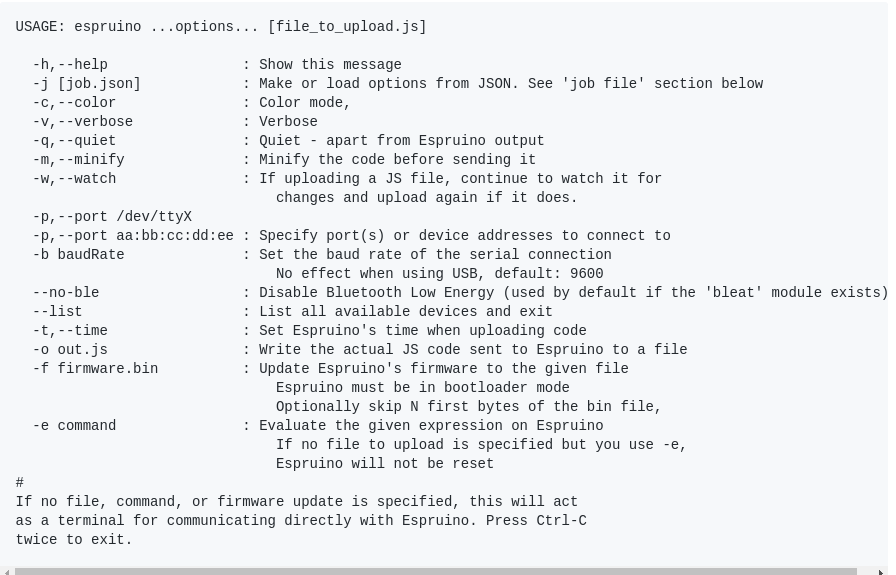
\includegraphics[width=15cm]{image/espruino_tools.png}
  }
  \caption{Espruino tools sous ligne de commande}
\end{figure}

\subsubsection{Esptools}
Esptools est un outil utilisé pour flasher différentes versions d’ESP, le chargement du micrologiciel ESPRUINO permet l'utilisation sur le ESP8266.\\
\begin{figure}[H]
  \centering
  \href{https://github.com/espressif/esptool}{
  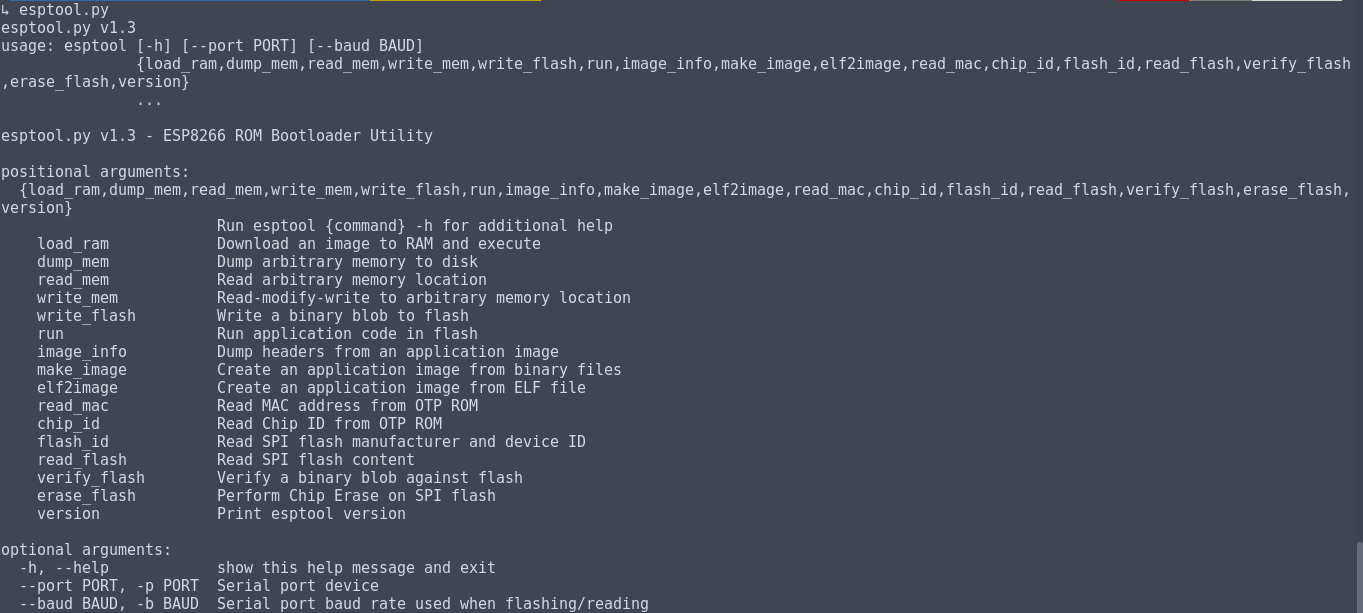
\includegraphics[width=15cm]{image/esptools.png}
  }
  \caption{Esptools}
\end{figure}
Il rend possible l'utilisation de JavaScript avec tous les microcontrôleurs supportés.\\
il est disponible également sous la forme d'un module \href{https://www.npmjs.com/package/esptool}{Node.js} pour les puristes de la ligne de commande.

\subsubsection{APISENSE}
La plate-forme APISENSE® permet de collecter une grande variété de données à partir des téléphones portables des usagers tout en garantissant le respect de leur vie privée. 
\begin{figure}[H]
  \centering
  \href{https://www.inria.fr/centre/lille/innovation/rii/rii-technologies-du-web/demos/apisense-r-accedez-a-une-foule-de-donnees-en-2-clics}{
  
\includegraphics[width=5cm]{image/apisense.png}
  }
  \caption{APISENSE}
\end{figure}

Utilisée dans de nombreux domaines, la plate-forme APISENSE® facilite la collecte, le stockage et le traitement des données renseignées par une foule d’usagers contributeurs. Basée sur les standards du web et déployée dans le Cloud, la plate-forme APISENSE® a notamment la capacité de traiter de gros volumes de données qui peuvent être restituées à différentes parties prenantes et sous différentes formes (OpenData, visualisations, etc.).



